\section{Design af spoler}\label{sec:sec_spole_design}
For at kunne dimensionere og designe en spole, er det væsentligt at vide hvilket formål spolen skal bruges til. Spolen har mange egenskaber, og i dette projekt vil de blive designet, så de kan bruges som sensorer. Altså en enhed der opfanger eller udsender et analogt signal. 

Som beskrevet tidligere, består systemet af i alt 3 spoler. 1 stor spole, som skal stå for at udsende et signal. Herudover 2 mindre identiske spoler, som skal opfange signalerne. For et illustrativt billede af opsætningen se afsnit **.
\husk{Simon}{Indsæt afsnitsnummer}

I den følgende tekst, vil der blive beskrevet hvilke faktorer der er blevet lagt vægt på, samt hvordan nogle af Maxwells ligninger er blevet brugt til at dimensionere de enkelte spoler. Herunder begreber som magnetfelt(B), flux$(\Phi)$, induktans(L) og elektromotorisk kraft som fremadrettet vil blive betegnet som EMF$(\xi)$. 

Først vil dimensioneringen af den store spole tages højde for, hvorefter der kigges på de 2 små spoler.
Den færdige dimensionering skal ende ud i et målbart EMF signal.

Der er som udgangspunkt blevet gjort brug af Biot-Savarts lov som ses i ligning \ref{eq:spole_biot_savart}.
\subsection{Magnetfelt}
\begin{figure}[h!]
	\centering
	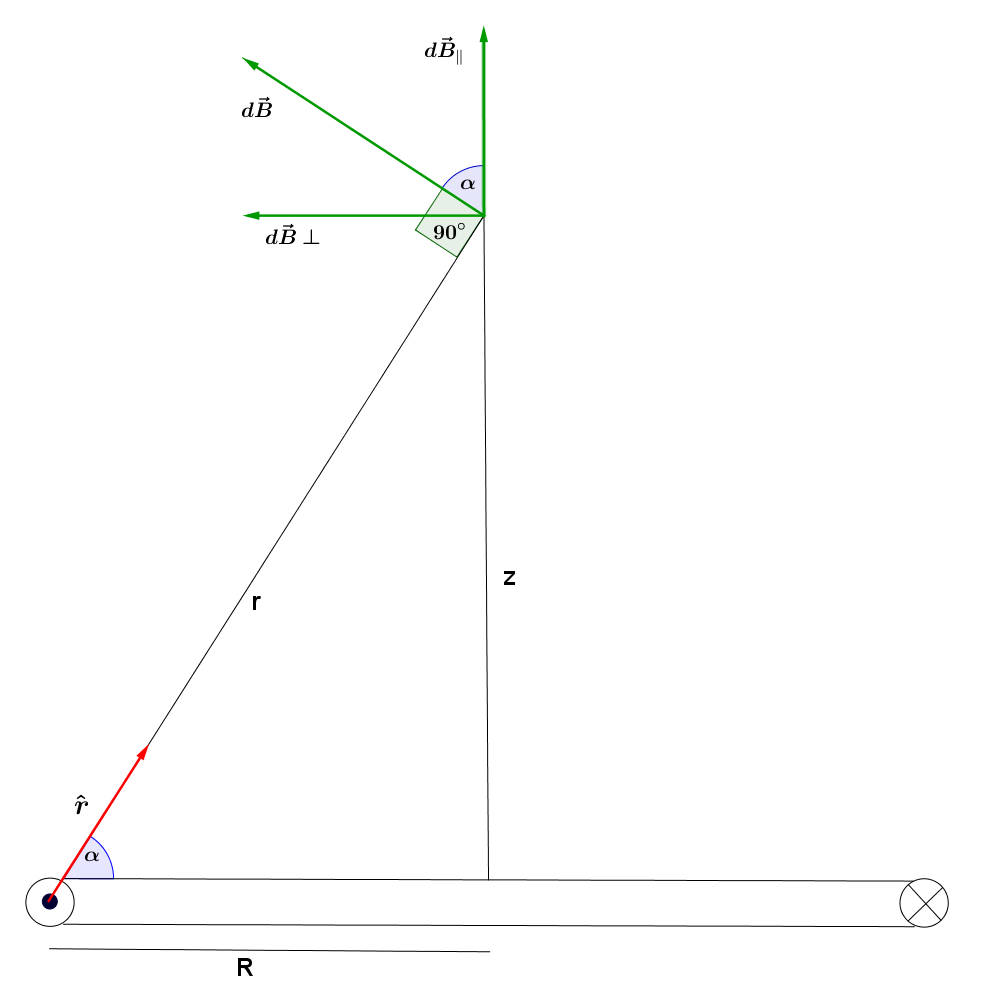
\includegraphics[width=.6\textwidth]{billeder/B_felt.png}
	\caption{Cirkulær leder med radius R}
	\label{fig:spole_fig1}
\end{figure}

På figur \ref{fig:spole_fig1} ses et tværsnit af en cirkulær leder, hvori der løber en strøm kaldet $i$. Krydset indikerer at stømmen går ind i papiret, og prikken også kaldet spidsen af en pil, indikerer at strømmen går ud af papiret. Man kan også se på denne figur, som den store spole med 1 vinding. Betragt punktet P på z aksen. I dette punkt ønskes et magnetfelts styrke bestemt, afhængig af positionen z. Som det ses er vinklen, uanset hvor på lederen man befinder sig, mellem $d\vec{s}$ og enhedsvektoren $\hat{r}$ altid $90\degree$ vinkeltret på hinanden.

Med dette kan $d\vec{B}$ feltet tegnes ind, vha. Biot-Savarts lov, eller vha. højrehåndreglen. En mere overskuelig måde at se det på er, at krydsproduktet af 2 vektorer, er en vektor der står vinkeltret på begge. 
$d\vec{B}$ kan nu deles op i 2 komposanter. En komposant $dB_\parallel$, som står parralelt på z axen og den cirkulære leder. Derudover også en komposant $dB_\perp$, som står vinkeltret på samme.

Summen af alle de vinkeltrette komposanter går ud da $d\vec{s}\times d\vec{B}_\perp=0$, og tilbage står kun de parallelle komposanter $dB_\parallel$, hvilket resulterer i:

 \begin{align}
 &B=\int dB_\parallel \label{eq:B_field}
 \end{align}

  
  
Betragt Biot-Savarts lov i ligning \ref{eq:spole_biot_savart}

\begin{align}
&d\vec{B}=\frac{\mu_0}{4\pi} \frac{i d\vec{s} \times \hat{r}}{r^2}\label{eq:spole_biot_savart}
\end{align}

Fra figur \ref{fig:spole_fig1}, kan ligning \ref{eq:spole_biot_savart} omskrives til:
\begin{align}
&dB=\frac{\mu_0}{4\pi} \frac{i ds\: sin(90\degree)}{r^2}\label{eq:spole_biot_savart2}
\end{align}
 Denne ligning giver udtryk for hvad det magnetiske felt er i en afstand $r$ fra $d\vec{s}$.
 
Ud fra figur \ref{fig:spole_fig1}, kan et udtryk for $dB_\parallel$ også vises.
 \begin{align}
 	&dB_\parallel=dB\: cos(\alpha)
 \end{align}
Hermed kan et samlet udtryk for $dB_\parallel$ gives: 
\begin{align}
&dB_\parallel=\frac{\mu_0 \:i\: cos(\alpha)\:ds}{4\:\pi\: r^2}
\end{align}
Da det er z der ønskes varieret, bliver et nyt udtryk nødt til at blive bestemt, hvor z indgår. Betragt figur \ref{fig:spole_fig1} igen. Her ses, at $r$ og vinklen $\alpha$, er relateret til hinanden, og ved hjælp at Phytagoras, kan disse 2 udtryk findes:
\begin{align}
&r=\sqrt{R^2+z^2} \\
&cos(\alpha)=\frac{R}{r}=\frac{R}{\sqrt{R^2+z^2}}
\end{align}

Da $i, R$ og $z$ alle har samme værdi for alle $ds$ hele vejen rundt i den cirklære leder, kan man vha. integration summere op, på samme måde som deffineret i ligning \ref{eq:B_field}, og der fås dermed et udtryk for B:
\begin{align}
&B=\frac{\mu_0 \: i \: R}{4\pi(R^2+z^2)^\frac{3}{2}}\int ds
\end{align}
Grænseværdierne for $\int ds$ er den cirkulære leders omkreds.
\begin{align}
&\int\limits_{0}^{2\pi R} ds = 2\pi R
\end{align}
Et endeligt udtryk for magnetfeltet $B(z)$ gives i ligning \ref{eq:Bz_field}.
\begin{align}
	&B(z)=\frac{\mu_0 \: i \: R^2}{2(R^2+z^2)^\frac{3}{2}} \label{eq:Bz_field}
\end{align}
Da dette udtryk kun er gældende for en cirkulær leder, altså en spole med 1 vinding, skal et nyt udtryk bestemmes. Dette udtryk tager udgangspunkt i ligning \ref{eq:Bz_field}, som blev udledt før.
\begin{figure}[h!]
	\centering
	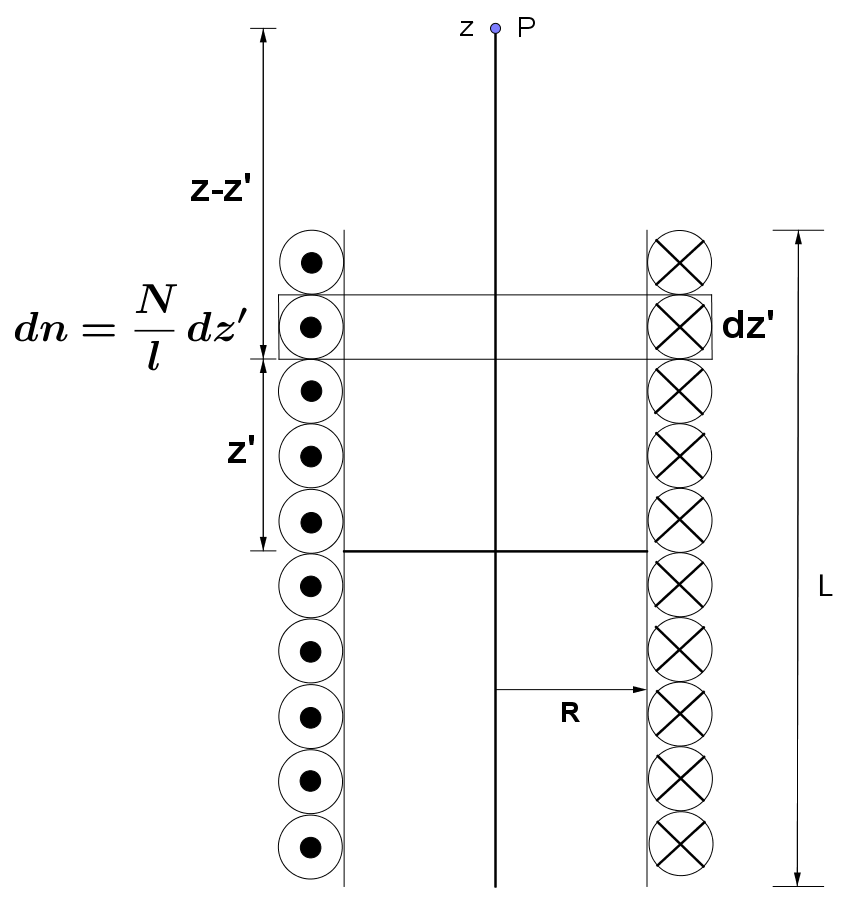
\includegraphics[width=.7\textwidth]{billeder/B_felt2.png}
	\caption{Solenoid med radius R}
	\label{fig:spole_fig2}
\end{figure}
Formlen for B feltet i en uendelig lang solenoid er givet ved:
\begin{align}
	&B=\mu ni
\end{align}
Hvor $n$ er antal vindinger pr. længde og udregnes ved $n=\frac{N}{L}$.
I dette udtryk er B feltet centreret i midten af den uendelig lange solenoide.

Da solenoidestørrelsen er bestemt, og ikke uendelig lang, samt $B$ feltet ligger uden for solenoidens yderkant, skal en ny ligning af $B$ feltet bestemmes.
Det antages at $B$ feltet er homogent omkring hele fladen, og ikke kun i det punkt der bestemmes.


Betragt figur \ref{fig:spole_fig2}. Her ses tværsnittet af en solenoide, med z aksen i centrum. Det ønskede $B$ felt skal bestemmes i punktet $P$.

Det ses at størrelsen af $dn$ er proportional med tykkelsen $dz'$:

\begin{align}
	&dn=\frac{N}{L} dz'
\end{align}



Ud fra ligning \ref{eq:Bz_field}, kan $dB(z)$ udtrykkes ved: 

\begin{align}
	&dB(z)=\frac{\mu_0 \: i \: R^2}{2(R^2+(z-z')^2)^\frac{3}{2}}dn=\frac{\mu_0 \: N \: i \: R^2}{2L(R^2+(z-z')^2)^\frac{3}{2}}dz'
\end{align}

Ved at integrerer over hele længden på solenoiden fås:

\begin{align}
	&B(z)=\int\limits_{-\frac{L}{2}}^{\frac{L}{2}}\frac{\mu_0 \: N \: i \: R^2}{2L(R^2+(z-z')^2)^\frac{3}{2}}dz'
\end{align}

Og et endeligt udtryk:
\begin{align}
	&B(z)= \frac{\mu_0 \: i \: N}{2L}\left(\frac{\frac{L}{2}-z}{\sqrt{(z-\frac{L}{2})^2+R^2}}+\frac{\frac{L}{2}+z}{\sqrt{(z+\frac{L}{2})^2+R^2}}\right) \label{eq:B_field2}
\end{align}
\subsection{Flux og elektromotorisk kraft}
I dette afsnit vil den magnetiske flux blive bestemt.  
Faraday lavede et eksperiment, og fandt ud af, at et magnetfelt der ændrer sig over tid i en lukket lederkreds, skabte en induceret EMF inde i kredsen.
Dette lavede han et udtryk for:
\begin{align}
	&EMF(\xi) = - \frac{d\Phi}{dt}
\end{align}
Denne lov er også kendt for navnet Lenz's lov, da han kom frem til det omvendte fortegn.

Flux i den lille spole hidrørende fra den store spole, ved fuld overlappelse er bestemt ved:
\begin{align}
	&\Phi_{21} = BA_2
\end{align}
Hvor $B$ er det magnetiske felt, og $A_2$ er arealet på den lille spoles overflade.
Da $B$ feltet er homogent på hele overfladen, antages $B$ konstant. 

Ud fra dette udtryk, kan den totale EMF, der er induceret over i den lille spole blive bestemt ved følgende udtryk:
\begin{align}
	&\xi = -N_2\frac{d\Phi_{21}}{dt} \label{eq:emf_lille_spole}
\end{align}
Hvor $N_2$ er antal vindinger i den lille spole.
Det er ikke nødvendigt at beregne den store spoles flux, i og med selvinduktansen kendes og dermed kan spændingen i den store spole findes ved:
\begin{align}
	&V = L\frac{di}{dt} \label{eq:ldidt}
\end{align}
\subsection{Strømfortrængning  og impedans}\label{Sec_skineff.}
I forbindelse med valg af trådtykkelse på kobbertråden, som skal vikles rundt om spolerne, er strømfortrængningen i ledningen væsentlig.\\
Hvis signalet i spolerne havde været et rent DC signal, kunne strømmen antages homogent i hele tværsnitsarealet i kobbertråden.
Da dette ikke er tilfældet, vil AC signalet "fotrænge" ud i kanten af kobbertrådens tværsnitsareal. 
Der bliver derved skabt et hulrum inden i kobbertråden. \\
Herved bliver modstanden i kobbertråden ændret.\\
En approximation af AC modstanden i kobbertråden findes ved ligning \ref{eq:R_AC}.
\begin{align}
	& R_{AC}=\frac{\rho l}{A_{eff}} \label{eq:R_AC}
\end{align}
Hvor $ \rho = \text{Resistiviteten i kobbertråden}$, $l = \text{Længden af kobbertråden}$, $A_{eff} =$ Det effektive areal af strømfortrængningen = $\pi r^2-\pi(r-\delta)^2$ og $r$ er radius på kobbertrådens tværsnit.

Frekvensen i spolerne, er dimensioneret forholdsvis høje, hvilket vil betyde strømfortrængning.
Formlen for strømfortrænging er givet ved ligning \ref{eq:skineffect}.
\begin{align}
	& \delta = \sqrt{\frac{\rho}{\pi f\mu_0\mu_r}} \label{eq:skineffect}
\end{align}
Hvor $f = \text{Frekvensen}$, $\mu_0 = \text{Permabilitetskonstant som er givet ved $4\pi 10^{-7}\henry/\meter$}$ og $\mu_r = \text{Den relative permabilitetskonstant for kobber}$.
\husk{Simon}{indsæt link som reference: http://chemandy.com/calculators/round-wire-ac-resistance-calculator.htm 5/12-16. kl 13}

\husk{Simon}{evt. henvis til https://mycableengineering.com/knowledge-base/conductor-resistance}

Dette gælder dog kun hvor $r>>\delta$. \\
Da kobbertråden er valgt meget tynd, vælges der efter analysering af strømfortrængningen at ses bort fra denne. 
I stedet findes impedansen for den store spole ved en given frekvens ved ligning \ref{eq:impedans}.
\begin{align}
	& Z=\sqrt{R^2+X^2} \label{eq:impedans}
\end{align}

Hvor $R$ er modstanden i spolen, og $X$ er reaktansen, som er givet ved:

\begin{align}
	& X=2\pi f L \nonumber
\end{align}
Hvor induktansen L for en solenoide er givet ved Wheelers formel i ligning\footnote{\url{http://microblog.routed.net/wp-content/uploads/2008/10/pancakewheel.pdf}} \ref{eq:Wheeler}
\begin{align}
	& L =\frac{31.6\cdot r_1^2\cdot N^2}{6\cdot r_1+9\cdot l + 10\cdot (r_2-r_1)}  \label{eq:Wheeler}
\end{align}
Et samlet udtryk for impedansen er dermed givet i ligning \ref{eq:impedans2}.

\begin{align}
	& Z=\sqrt{\left(\frac{\rho l}{A_1}\right)^2+\left(2\pi f L\right)^2} \label{eq:impedans2}
\end{align}


\subsection{Resultater}
I følgende afsnit vil den teoretiske del blive anvendt, til at eftervise teorien i praksis.\\
Der vil blive gjort rede for de forskellige dimensioneringer og valg - derudover, vil målinger foretaget med et oscilloskop blive analyseret.\\ 
Resultaterne vil blive delt op i undersektioner, så hvert emne passer i rækkefølge med kapitlet.\\
Igennem hele kapitlet, antages det at strømmen $i$ er givet ved:
\begin{align}
	 i&=0.05\sin{(2\pi46936 t)} \nonumber
\end{align}
Med mindre andet er angivet.\\
Denne strøm er givet ved, hvordan det virkelige system ville opføre sig rent teoretisk, uden støj og andre forstyrrelser.
Derudover er der i alle laboratorieopstillinger, sat en $1\ohm$ modstand i serie med den store spole, for at kunne detektere den angivne strøm i spolen.
Have in mente, at frekvensgeneratoren i afsnit \ref{sec:frekv_gen} laver et $\textbf{firkantsignal}$.\\ 
Hele teorien afhænger af spolernes fysiske design, derfor er disse dimensioneret på forhånd, og kan ses i afsnit \ref{sec:3D_design}.

%\begin{align}
%	i &= 0.05\cdot \sin{(2pi\cdot 46936\cdot t)} \nonumber \\
%	\mu_0 &= 4\pi 10^{-7}T\cdot \m/A \nonumber \\
%	l &= 0.01\m \nonumber \\
%	\text{Trådtykkelse} &= 0.00025\m \nonumber\\
%	N_1&=63\nonumber\\
%	N_2&=300\nonumber\\
%	R_1&=0.0175\m\nonumber\\
%	R_2&=0.00855\m\nonumber\\
%	A_1&=9.6211\cdot 10^{-4} \m^2\nonumber\\
%	A_2&=2.2966\cdot 10^{-4} \m^2\nonumber
%\end{align}
\subsubsection{Magnetfelt}
Magnetfeltet er dimensioneret $13\mm$ ud fra den store spoles centrum.
Det antages at magnetfeltets størrelse er homogent i alle punkter i dette spektrum.
Dette svarer præcist til centrum af modtagerspolerne ved fuld overlappelse.\\
Da magnetfeltet afhænger meget af strømmens størrelse og antal vindinger, bliver der dimensioneret ud fra dette.
Kobbertråden der er valgt, har en diameter på $0.25\mm$.
Dette gælder både for den store og de to små spoler.
Da der ønskes så lidt tab, i overførelsen mellem sender og modtagerspole, anvendes Faradays lov, til at bestemme viklingsforholdet.
Der er taget udgangspunkt i ligning \ref{eq:emf_lille_spole}, hvor det ses at vindingstallet er proportionalt med ændring i fluxen.
Derfor vælges $N_2>>N_1$, hvor $N_1 = 63$ og $N_2 = 300$.

Hvilket giver en trådlængde på hhv.:
\begin{align}
	\text{Trådlængde stor spole} & \approx 7\m  \nonumber \\
	\text{Trådlængde lille spole} & \approx 16\m \nonumber
\end{align}

Strømmen vælges forholdsvis lav, da kobbertråden er meget tynd, hvilket resulterer lav modstand. 
Dog ønskes så høj strøm som muligt, da modtagerspolerne gerne skulle kunne registrerer et signal.\\
Peakstrømmen i den store spole vælges derfor til $I_{Peak} = 0.05\si{\ampere}$.

I figur \ref{fig:B_felt_stor_spole}, ses et plot over magnetfeltet, der ændrer sig i form af en sinus, hvor tiden varierer.
Det ses, at $13\mm$ ud fra den store spole, skulle kunne måles et $B$ felt på ca. $60\micro\tesla$.\\
\begin{figure}[h!]
	\centering
	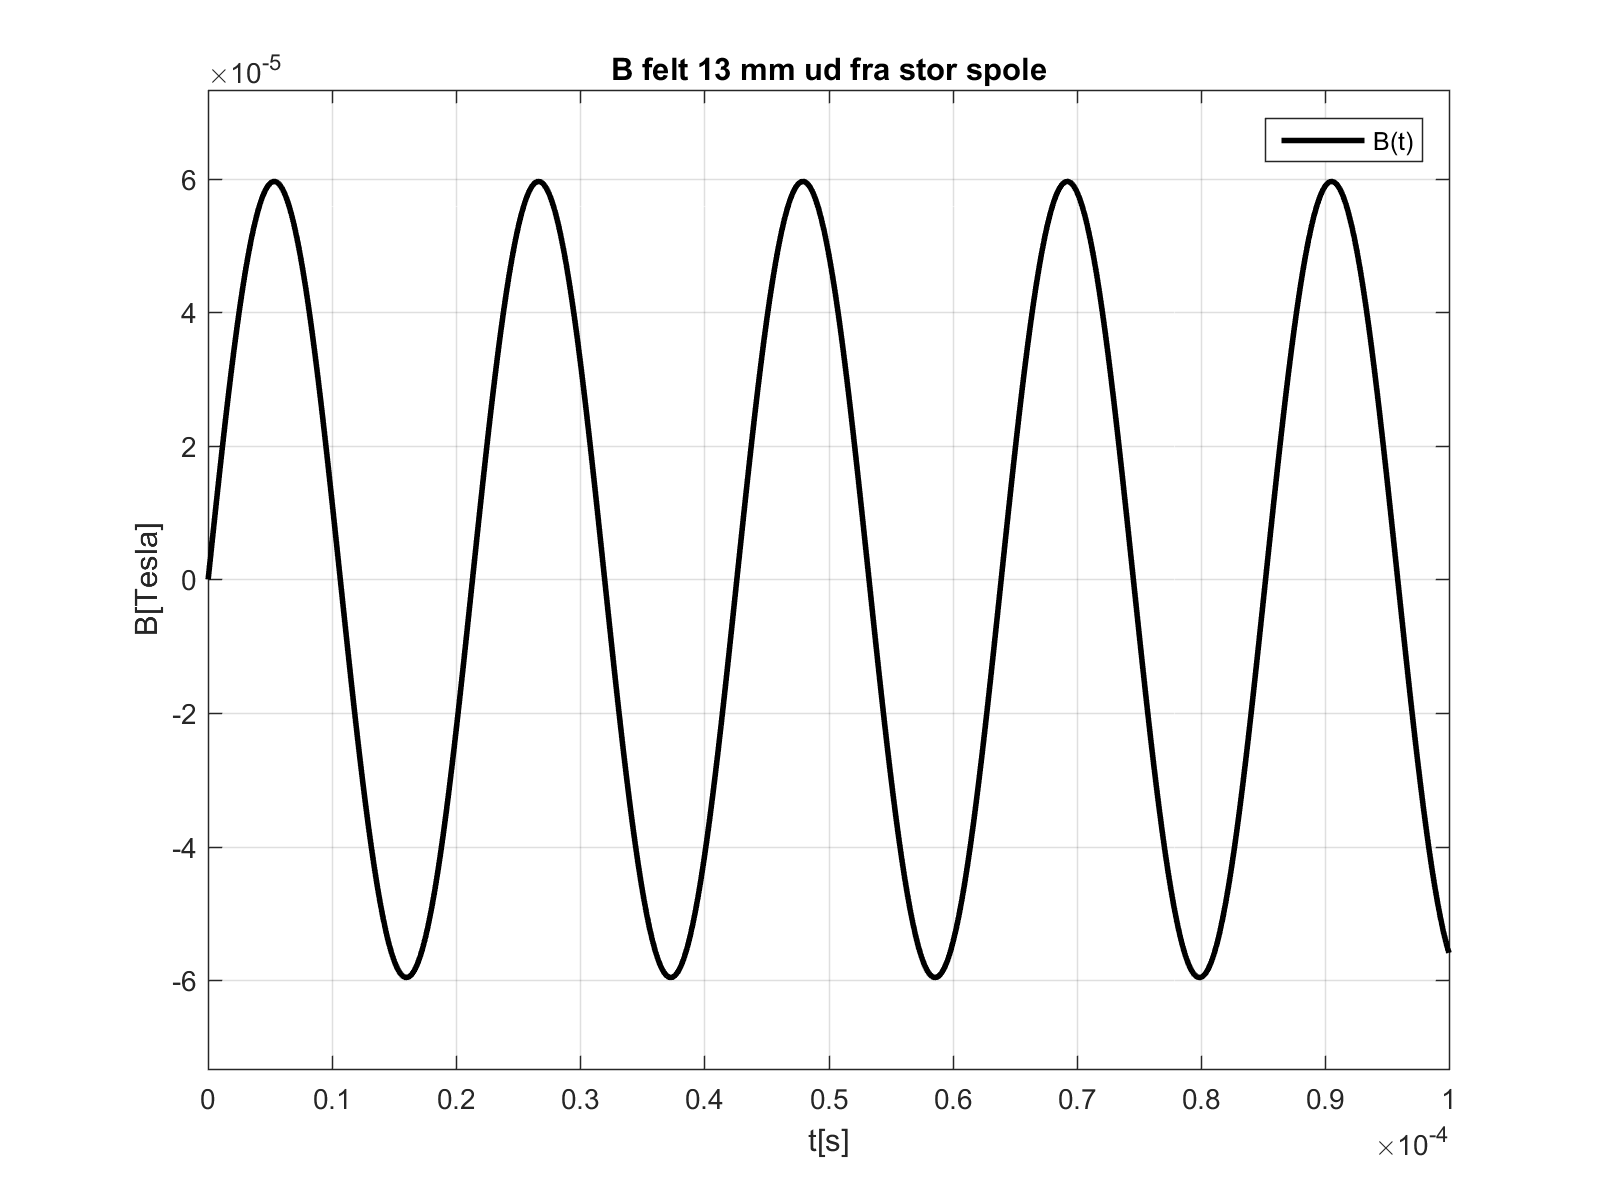
\includegraphics[width=1\textwidth]{billeder/B_felt_stor_spole.png}
	\caption{Magnetfeltet beregnet 13 $\mm$ ud fra stor spole. Funktionen til grafen ses i ligning \ref{eq:B_field2}.}
	\label{fig:B_felt_stor_spole}
\end{figure}\\
For at eftervise dette, blev der i laboratoriet, målt med et Gauss meter af typen. \husk{Simon}{Find ud af type}
Med en konstant strøm på $0.05\ampere$ igennem den store spole, blev der målt $0.5 \gauss$ ca. $13\mm$ ud fra spolens centrum. 
Dette svarer til $50 \micro\tesla$. 
Ses der på figur \ref{fig:B_felt_stor_spole}, er der et peak magnetfelt på ca. $60\micro\tesla$.
Da jordens magnetfelt\footnote{\url{https://en.wikipedia.org/wiki/Earth's_magnetic_field}} i sig selv, ligger mellem $25-65\micro\tesla$, kan denne måling ikke antages fuldstændig præcist.

\subsubsection{Flux og elektromotorisk kraft}
Efter at have bestemt magnetfeltets styrke, i forrige afsnit, kan den magnetiske flux og den elektromotoriske kraft bestemmes.\\
I det virkelige system, vil spændingssignalet i den store spole, være et firkant signal.
Da dette ikke kan eftervises på nogen nem måde i MatLab, tages der udgangspunkt i et sinussignal.
Dette laves også i laboratoriet vha. af en funktionsgenerator.
På den måde kan teorien bedst sammenlignes med praksis.\\
Betragt figur \ref{fig:EMF_spole}, her ses to grafer.
Den røde indikerer spændingen over den store spole.
Den blå indikerer spændingen over den lille spole, vel og mærke ved fuld overlappelse af arealerne på hhv. stor og lille spole.\\
Det ses, at i følge Faradays lov, skal peakspændingen i den lille spole ligge på ca. $1.2\volt$.
Dette vil nu eftervises i laboratoriet.

\begin{figure}[h!]
	\centering
	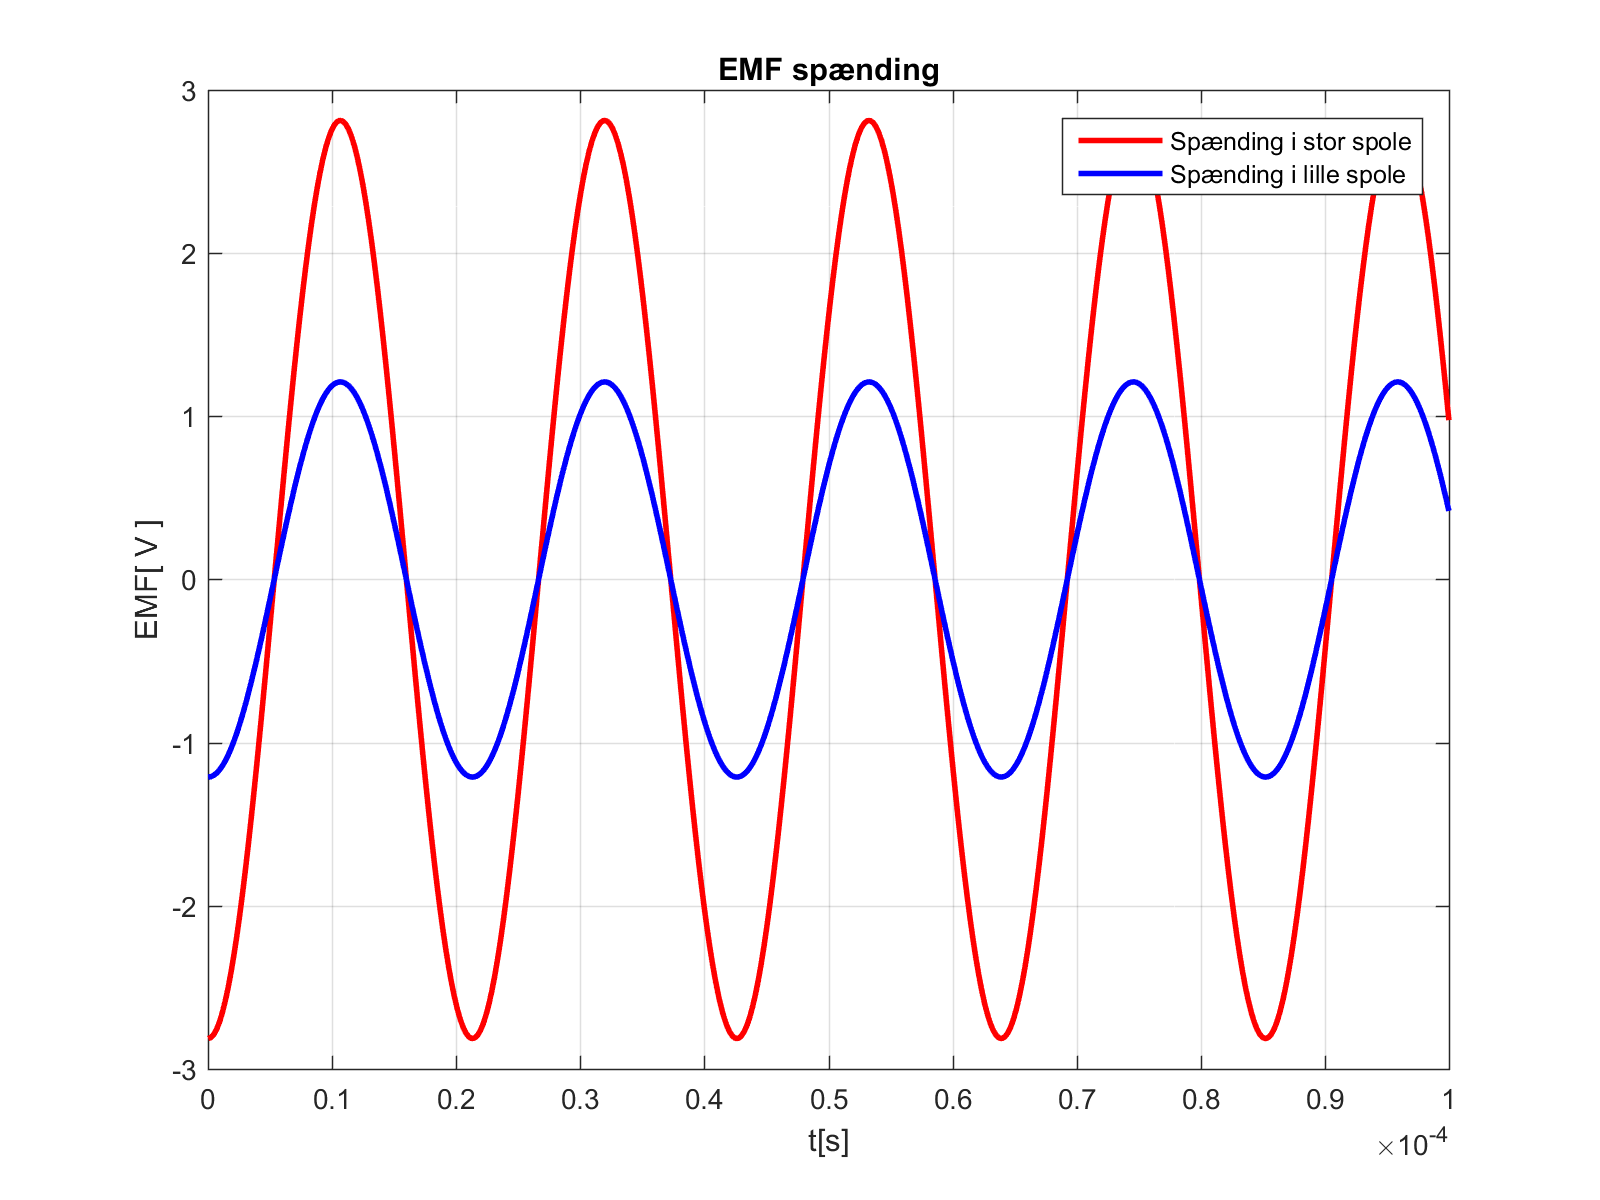
\includegraphics[width=1\textwidth]{billeder/EMF_spanding.png}
	\caption{EMF spænding i stor og lille spole}
	\label{fig:EMF_spole}
\end{figure}

I laboratoriet opstilles et kredsløb, som vist på figur \ref{fig:kredslob_spole}, hvor den store spole er blevet målt med et LCR meter, og har en induktans på $205\micro\henry$.
Det er ønskeligt at have en peakstrøm på $0.05 \ampere$, som i teorien.\\
På funktionsgeneratoren, er der en udgangsimpedans på $50\ohm$.
I serie med resten af kredsløbet, sidder en $1\ohm$ modstand. Spændingen over denne ønskes bestemt til $0.05\volt$, hvilket vil give de ønskede $0.05\ampere$ igennem spolen.
Vha. af spændingsdeling og ligning \ref{eq:impedans}, bestemmes funktionsgeneratorens amplitude til $3.9\volt$.\\
Resultatet af dette, bliver som vist i figur \ref{fig:EMF_spole_lab}.
Hvor den gule kurve, er spændingen over den store spole, og den grønne kurve er spændingen over den lille spole.\\
Sammenligner man figur \ref{fig:EMF_spole_lab} med \ref{fig:EMF_spole}, ses en tydelig sammenhæng.\\
\begin{wrapfigure}{r}{0.5\textwidth}
	\centering
	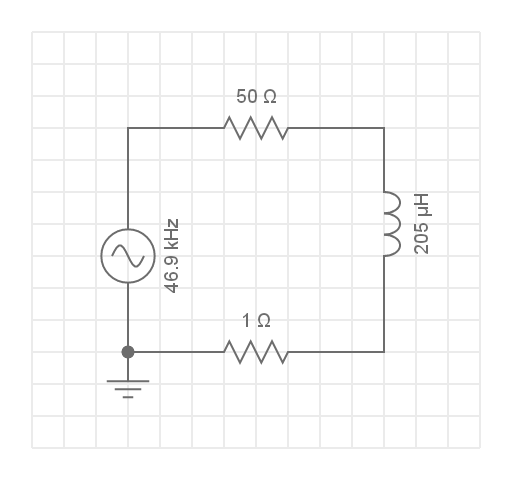
\includegraphics[width=.5\textwidth]{billeder/circuit_spole.png}
	\caption{Laboratorieopstilling med $1\ohm$ modstand i serie, for at måle strømmen}
	\label{fig:kredslob_spole}
\end{wrapfigure}
EMFen i den lille spole i praksis, er ca. $0.25\volt$ fra teorien.\\ \\
Disse resultater stemmer overens med hvad der blev beregnet i teorien. Da der blev benyttet en frekvensgenerator med et sinussignal i beregningerne, antages det at det er det samme med et firkantsignal. \\

\begin{figure}[h!]
	\centering
	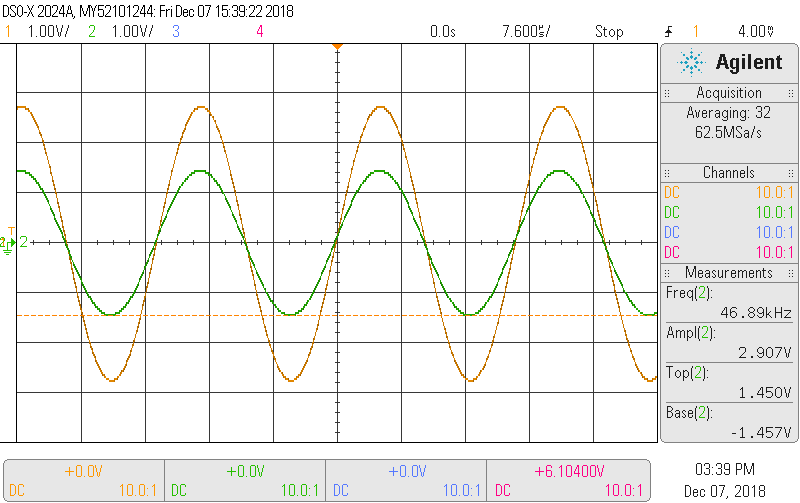
\includegraphics[width=1\textwidth]{billeder/vin_vout_png.png}
	\caption{EMF spænding i stor og lille spole, målt i laboratorie}
	\label{fig:EMF_spole_lab}
\end{figure}
\newpage
\subsubsection{Strømfortrængning og impedans}
Tykkelsen på kobbertråden, er som skrevet valgt meget tynd.
Der kan derfor ses bort fra strømfortrænging.\\
I stedet er induktansen og impedansen blevet målt og beregnet.\\
Induktansen er beregnet ud fra ligning \ref{eq:Wheeler}.

\begin{align}
	 L_{beregnet} &= 192.04\micro\henry\\
     L_{\text{målt}} &= 205\micro\henry
\end{align}

Impedansen i den store spole, er beregnet ud fra ligning \ref{eq:impedans2}
\begin{align}
	 Z_{\text{beregnet-100k\hertz}}&=120.69\ohm\\
	 Z_{\text{målt-100k\hertz}}&=129.3\ohm\\
	 Z_{\text{beregnet-46.9k\hertz}}&= 56.7\ohm               
\end{align}

\subsection{3D design/fysisk design af spolehus}\label{sec:3D_design}
For at kunne gøre disse spoler til en realitet, er der lavet specialdesignede spolehuse som passer perfekt til de udregnede værdier. Disse spoler er blevet tegnet i 3D-CAD programmet Inventor, og derefter 3D-printet på en 3D-printer. \\

Spolerne er designet således at når den store spole er i nul (i midten) overlapper den de mindre spoler så de er dækket præcist 50\percent. Når den store spole så er i sin fulde udslagsvinkel er hhv. den ene mindre spole dækket helt, hvor den anden slet ikke er dækket. \\

Disse spoler er designet med brugervenlighed i bagtankerne. For at vi ikke skal designe et nyt spolehus for hver gang vi vikler en ny spole, er der lavet et Plug-n-play system hvor kan nemt kan "klikke" nye spoler i. Dette er lige så meget for at undgå spild af filament. Derudover er der lavet huller, så det er nemt at putte dem i vindingsmaskinen. \\

Da basen af køretøjet er noget der er taget fra et tidligere projekt, er spolerne lavet sådan, at de nemt er til at klikke på det nuværende pendul, samt køretøjets bundplade. (Det gennemsigtige på figur \ref{fig:spole_3d_fig} er resten af bilen.)

\begin{figure}[h!]
	\centering
	\subbottom[]{%
		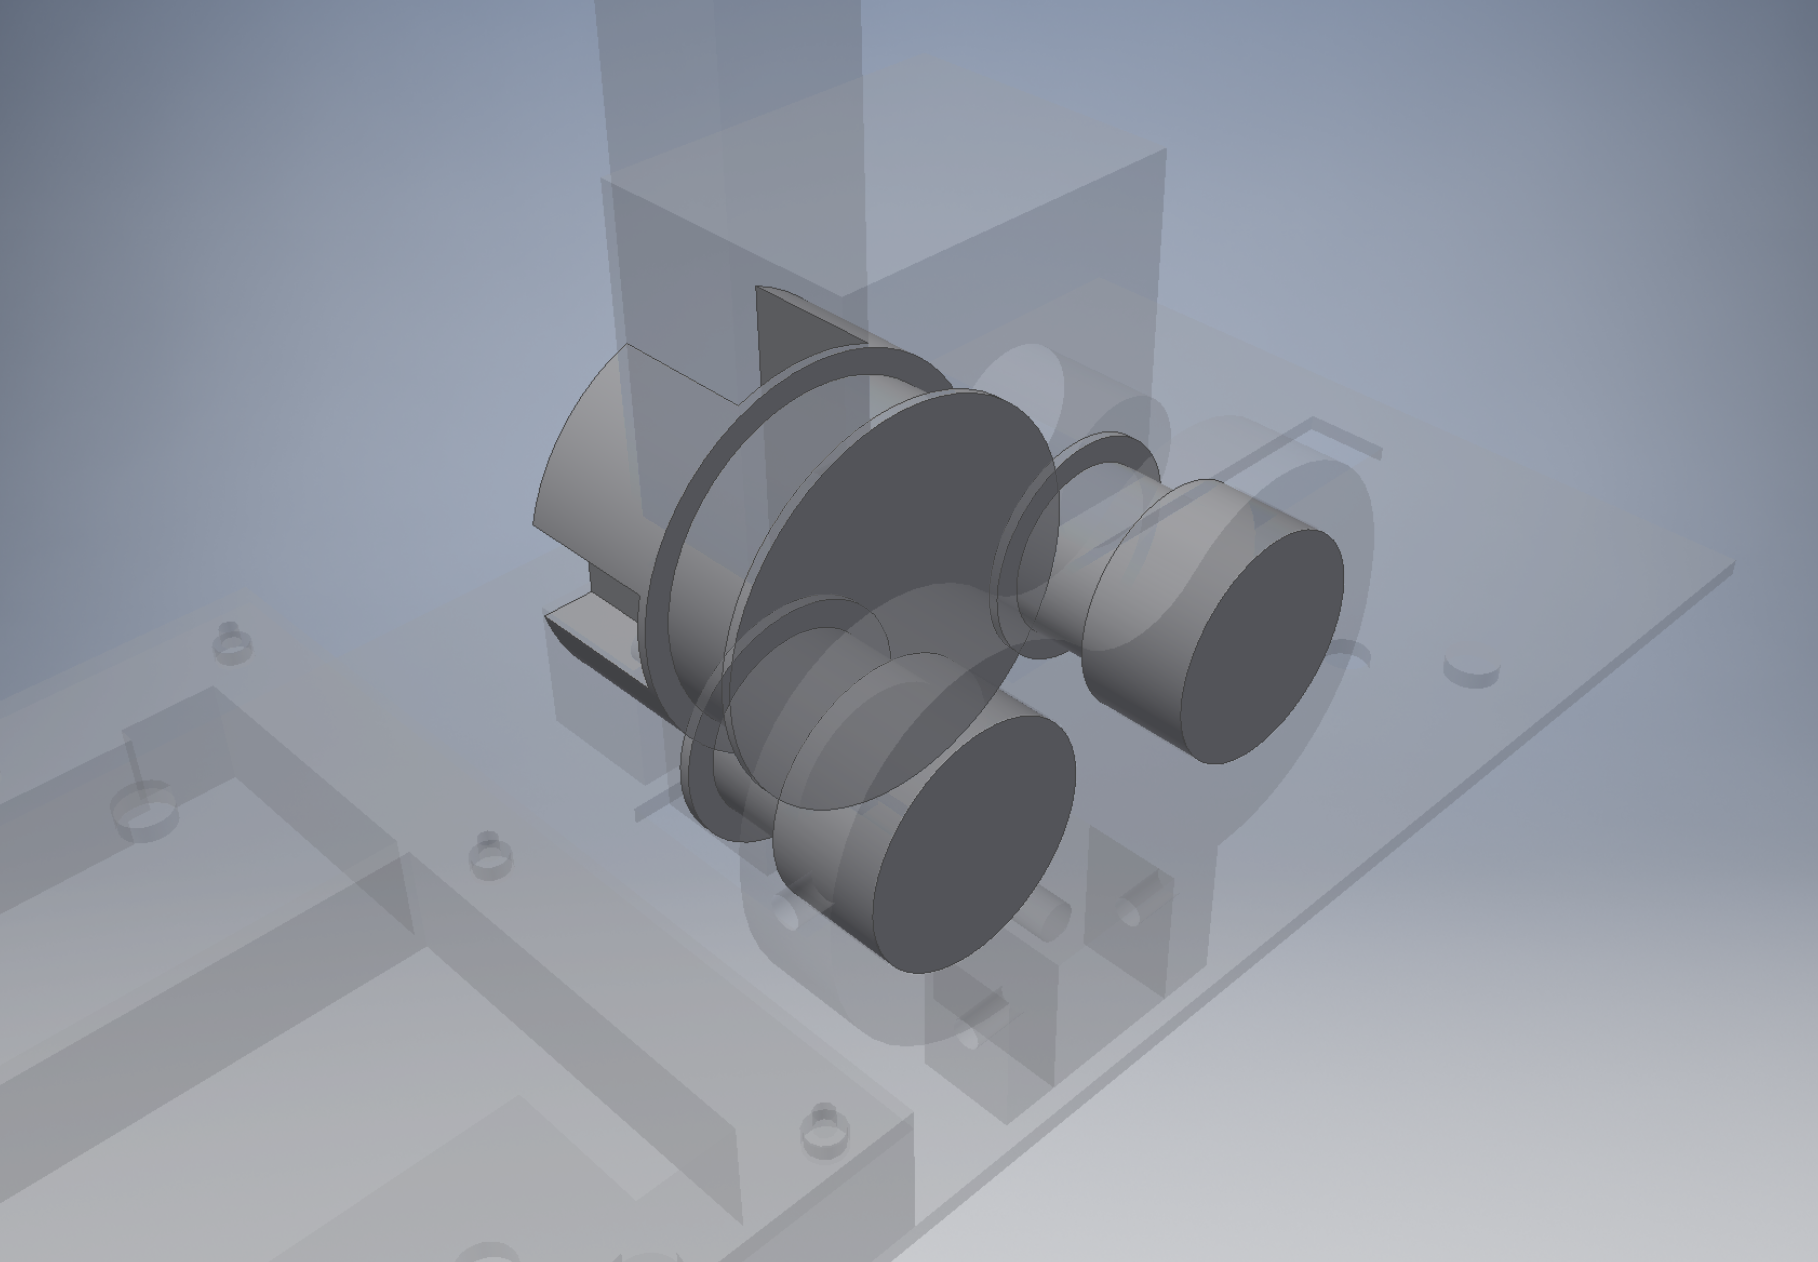
\includegraphics[width=.49\textwidth]{billeder/spoler_3d.png}
		\label{fig:spole_3d_fig}}
	\subbottom[]{%
		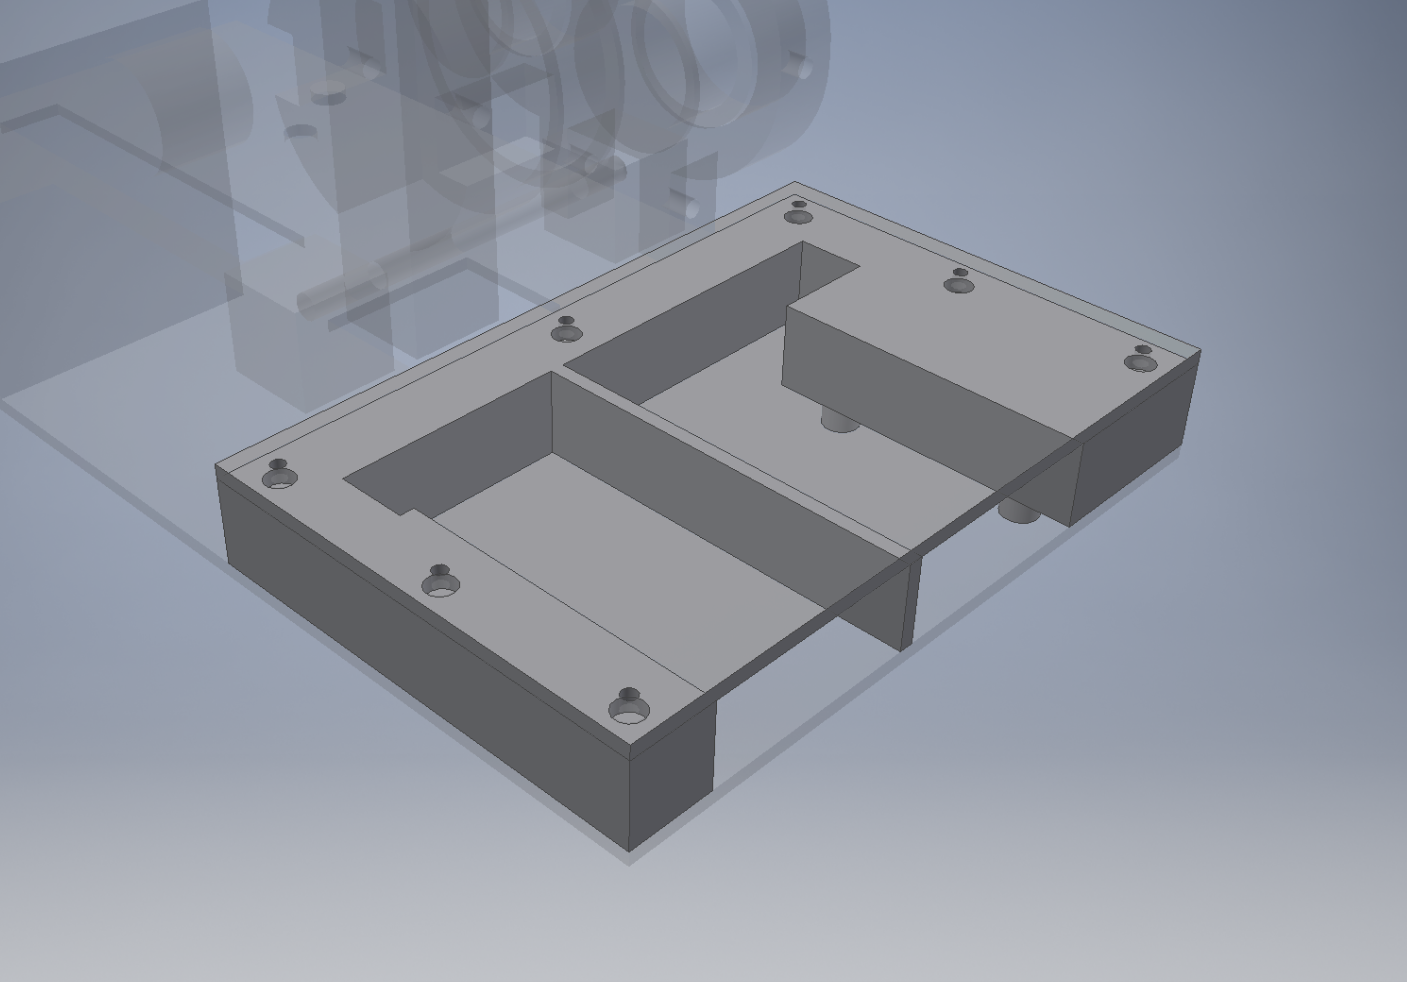
\includegraphics[width=.49\textwidth]{billeder/printmount_3d.png}
		\label{fig:printmount_3d}}
	\caption{De 3 spoler (a), samt batteriholder og printmount (b).}
\end{figure}

\subsection{Afsenderspolen}
Den store spole (afsenderspolen) har følgende mål; 
Diameteren er $35\milli\meter$, og dens dybde er $10\milli\meter$. Derudover har den en kant på $2.5\milli\meter$ så der er plads til tråden. Tykkelsen på denne kant er $1\milli\meter$. 

\subsection{Modtagerspolerne}
De små spoler (modtagerspolerne) har følgende mål; 
Diameteren er $17.1\milli\meter$, og dens dybde er også $10\milli\meter$. Kanten er den samme som på afsenderspolen. Centrum af disse spoler er på linje med ydrekanten af den store spoles $35\milli\meter$ da vi på denne måde opnår den største følsomhed. \\

Derudover er der designet en batteriholder samt printmonteringsplade som også udnytter de nuværende huller i bilens bundplade. Batterierne kan slides ind i to holdere under printet, så stikkene kan gå direkte op i printet. Se figur \ref{fig:printmount_3d}.\\
